% Benchmark Evaluation Section

In order to verify and demonstrate the capabilities of the CircusTent benchmark suite, we conducted an evaluation of a diverse set of platforms with respect to atomic memory operations.
In the interest of space, and in order to provide a comprehensive introduction to CircusTent and its constituent kernels in Section~\ref{sec:circustent}, we evaluated only our OpenMP backend in this work.
The evaluation of other backend implementations is left for a future work.
We first introduce our test platforms and briefly describe pertinent details of their architecture in Section~\ref{subsec:platforms}.
We next detail our evaluation methodology in Section~\ref{subsec:methodology}.
Results for each of the CircusTent benchmark kernels are presented in Section~\ref{subsec:results}.
Finally, we analyze and discuss observed patterns and performance characteristics in Section~\ref{subsec:analysis}.

\subsection{Platforms}
\label{subsec:platforms}

We evaluate CircusTent across a total of fourteen distinct platforms that encompass device classes ranging from embedded systems to those used in petascale-class supercomputers.
These systems feature single and dual socket configurations utilizing processors from Intel, AMD, and ARM with varied instruction set architectures, clock frequencies, and core counts.
Similarly, the total memory capacity differs across platforms.
Table~\ref{tab:benchsys} provides an overview of our test platform specifications wherein each system is denoted by its processor model.
The size of the \texttt{VAL} array used during our evaluation, as well as the compiler used to build CircusTent, is also shown for each platform.

As the organization of each system's cache hierarchy is an important factor to its benchmark performance, some further detail in this regard is warranted.
Many of the processors featured in our test platforms adhere to a somewhat standard cache hierarchy design.
Each of these processors feature a three-level hierarchy wherein the L1 and L2 caches are private to each core and the L3 caches are shared between cores in a given socket.
Each L1 cache is subdivided into L1i and L1d caches for instructions and data, respectively.
For the sake of brevity, we detail only systems whose cache organization deviates from this norm, and how they do so, below.

\begin{itemize}
\item Cortex-A53 -  The Arm Cortex-A53 is hosted on a Raspberry Pi Model 3B+.
This model features four cores, each with a private 32KiB L1 cache and a 512KiB shared L2 cache.
The Cortex-A53 does not have any cache levels beyond L2.
\newline
\item Cortex-A72 - Similar to the A53, the A72 has two cache levels.
The L1 cache is split between a 32KiB instruction cache and a 48KiB data cache.
The 1MiB L2 cache is shared amongst all the cores with no further caching layers.
\newline
\item Ryzen V1605B - The AMD Ryzen V1605B embedded x86\_64 socket is hosted via an Udoo Bolt platform.
The processor features an L1 cache split between a 256KiB instruction cache and a 128KiB data cache.
The L1 instruction cache is 4-way set associative and the data cache is 8-way set associative.
The L2 cache is 2MiB using an 8-way set associative configuration.
The L3 cache is also 8-way set associative with 4MiB of capacity.  
\newline
\item Core i7-4980HQ - In addition to a conventional 6 MiB L3 cache shared between cores, this processor also features a 128 MiB eDRAM L4, or ``Crystal Well", cache that is shared between the CPU cores and the integrated GPU.
\newline
\item Xeon Phi 7250 - The 68 cores present in this processor are arranged in 34 tiles of 2 cores each.
Herein, cores coresident within a tile share a 1MiB L2 cache.
Although it does not incorporate a true shared last level cache, this processor features 16 GiB of MCDRAM that can be used as addressable memory, a shared cache across all cores, or in a hybrid configuration. 
For our evaluation, the MCDRAM is utilized in the cache configuration.
\end{itemize}

\begin{table*}
\caption{Benchmark System Configurations}
\label{tab:benchsys}
\begin{tabular}{ccp{10mm}cp{15mm}ccp{16mm}c}
\toprule
System&Clock Frequency&Cores / \newline~Socket&Total Sockets&LLC Size\newline~/ Socket&Total Memory&Array Size&Operating\newline System&Compiler\\
\midrule
Cortex-A53      & 1.40Ghz & 4  & 1 & 512KiB  & 512MiB & 256MiB  & Ubuntu\newline 18.04 4.15.0 & GCC 7.4.0\\
Cortex-A72      & 1.50Ghz & 4  & 1 & 1MiB   & 4GiB & 256MiB  & Debian\newline 10.1 4.19.75 & GCC 8.3.0\\
Ryzen V1605B    & 1.58Ghz & 4  & 1 & 4MiB    & 32GiB & 15GiB & Ubuntu\newline 19.04 5.2.10&GCC 8.3.0\\
Opteron 4130    & 2.60Ghz & 4  & 2 & 6MiB   & 64GiB & 15GiB & Centos7\newline 3.10.0&GCC 8.3.1\\
Core i5-3210M   & 2.50Ghz & 2  & 1 & 3MiB   & 4GiB & 256MiB & macOS\newline 10.13.6&clang 9.1.0\\
Core i7-3930K   & 3.20Ghz & 6  & 1 & 12MiB  & 64GiB & 15GiB & Linux Mint\newline 18.3 4.15.0&GCC 5.4.0\\
Core i7-4980HQ  & 2.80Ghz & 4  & 1 & 6MiB L3 +\newline 128MiB L4 & 16GiB & 15GiB & macOS\newline 10.15.3&GCC 9.2.0\\
Xeon Phi 7250   & 1.40Ghz & 68 & 1 & 16GiB \newline MCDRAM & 96GiB & 15GiB & SLES\newline 4.12.14&GCC 8.3.0\\
Xeon E5620      & 2.40Ghz & 4  & 2 & 12MiB & 48GiB & 15GiB & Ubuntu\newline 16.04 4.4.0&GCC 5.4.0\\
Xeon X5650      & 2.67Ghz & 6  & 2 & 12MiB & 64GiB & 15GiB & Ubuntu\newline 18.04 4.15.0&GCC 7.5.0\\
Xeon E5-2620 v3 & 2.40Ghz & 6  & 1 & 15MiB & 64GiB & 15GiB & Ubuntu\newline 16.04 4.4.0&GCC 5.4.0\\
Xeon E5-2670 v2 & 2.50Ghz & 10 & 2 & 25MiB & 64GiB & 15GiB & Centos7\newline 3.10.0&GCC 7.3.0\\
Xeon E5-2695 v4 & 2.10Ghz & 18 & 2 & 45MiB & 192GiB & 15GiB & Centos7\newline 3.10.0&GCC 7.3.0\\
Xeon E5-2698 v3 & 2.30Ghz & 16 & 2 & 40MiB & 128GiB & 15GiB & SLES\newline 4.12.14&GCC 8.3.0\\
\bottomrule
\end{tabular}
\end{table*}

\subsection{Methodology}
\label{subsec:methodology}

Consistent with previous studies \cite{villa2008barriers}\cite{david2013sync}\cite{schweizer2015evaluating}\cite{hoseini2019modeling}, we perform our initial evaluation of the CircusTent suite in the context of a physically shared memory environment.
In order to do so, we execute each of the CircusTent benchmark kernels, detailed in Section~\ref{subsec:algorithms}, on the test platforms introduced above using our OpenMP backend.
For each kernel, we conduct trials using implementations based on both the atomic \textit{Add} and \textit{Compare-and-Swap} primitives.
A uniform stride size of $N=9$ is utilized for each trial of the StrideN kernel.

We collect performance results for each platform.
In order to eliminate any performance volatility associated with simultaneous multithreading, we vary the thread count during our trials from a single thread, up to one thread per physical core, for each platform.
Similarly, 64-bit operands are used throughout the evaluation to prevent any inconsistencies.
Moreover, to better simulate real-world behavior, we allow the operating system and programming model to perform the mapping of threads to processor cores.

Where feasible, a uniform size of approximately 15 GiB is utilized for the \texttt{VAL} array on each platform.
For the Cortex A-53, Cortex A-72, and Core i5-3210M systems, wherein physical memory limitations make this configuration impractical, a 256 MiB \texttt{VAL} array is utilized instead.
In order to generate sufficient runtime such that observable patterns of behavior emerge, twenty million iterations of each kernel loop are run during every benchmark trial.
We utilize our normalized \textit{GAMs} metric, as introduced in Section~\ref{subsec:normalizingtheresults}, throughout our evaluation to measure and compare the performance of our diverse set of test platforms.

\subsection{Results}
\label{subsec:results}

\subsubsection{Random Access}
\label{subsubsec:random_access_res}

\begin{figure}[!t]
\centering
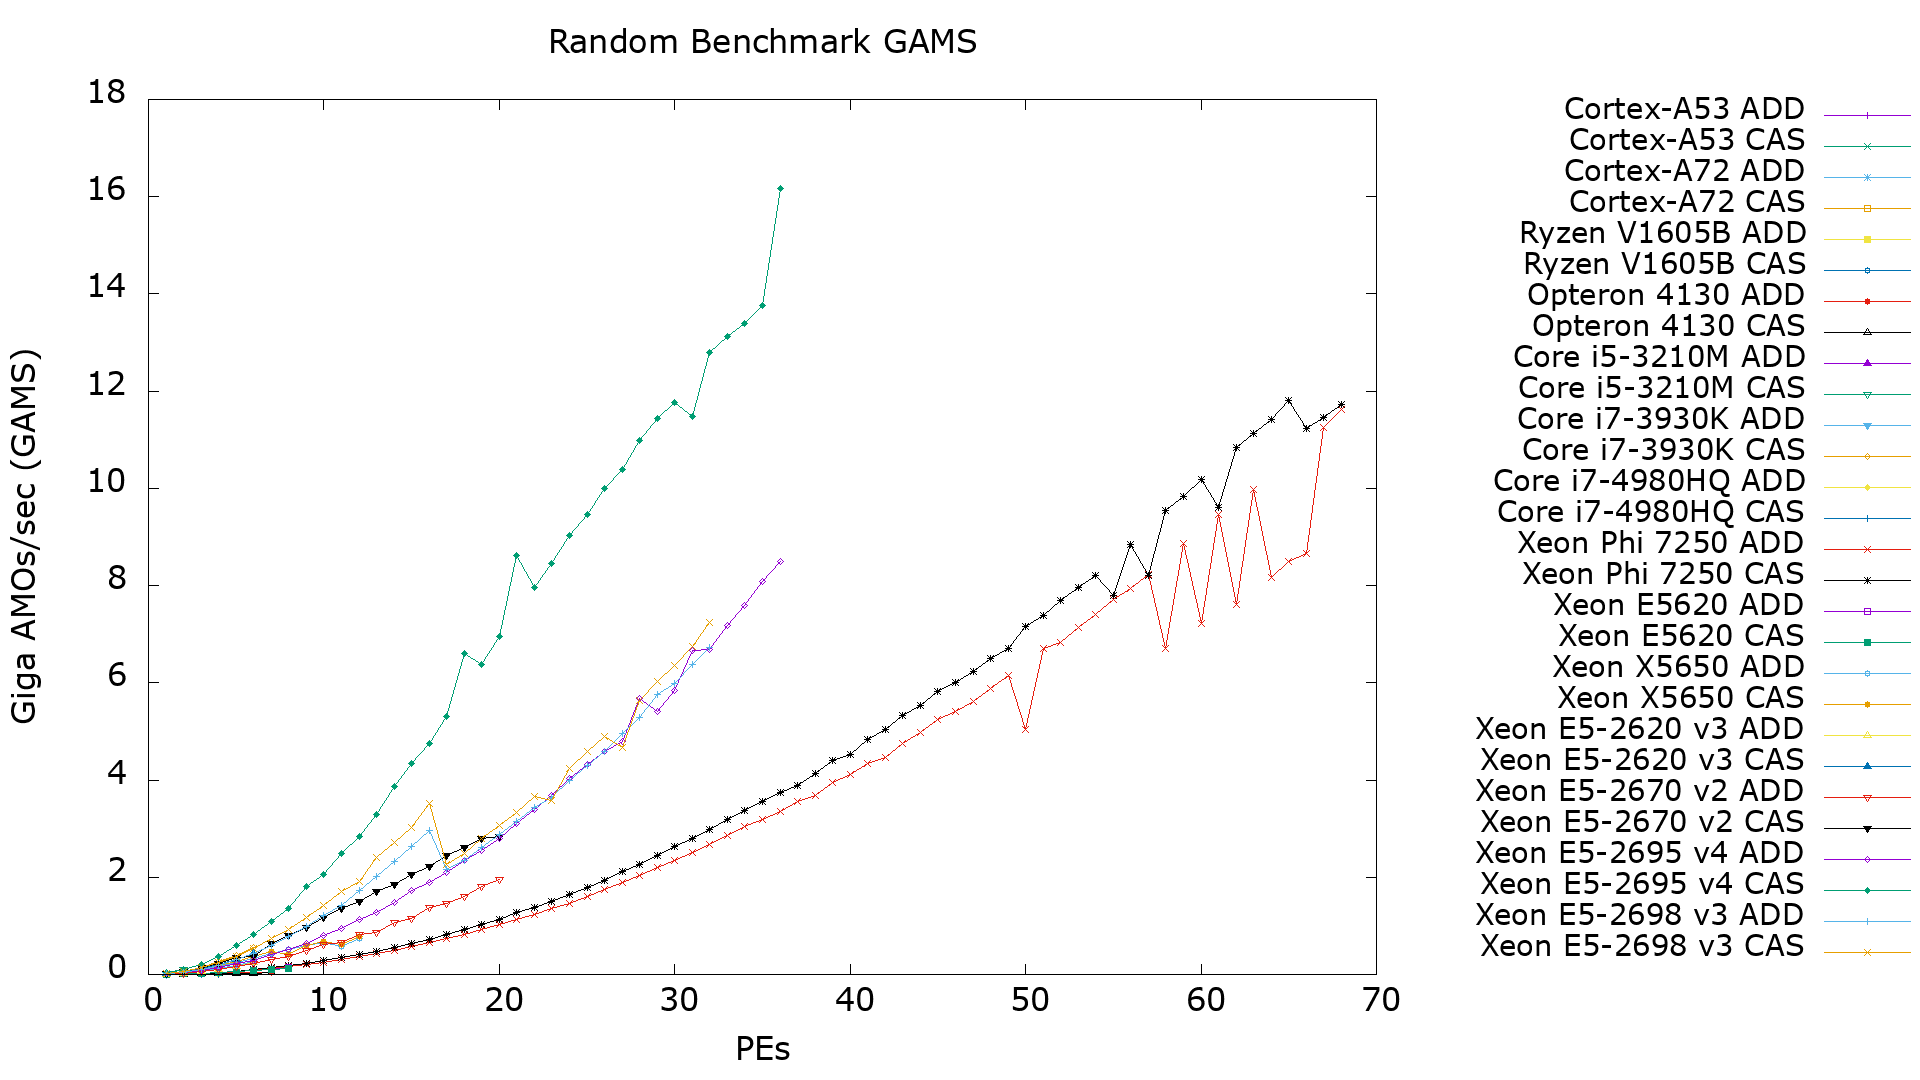
\includegraphics[width=3.5in]{figures/RAND_GAMS.png}
\caption{Random Benchmark GAMS}
\label{fig:rand_gams}
\end{figure}

We first examine our benchmark results from the Random Access kernel as shown in Figure~\ref{fig:rand_gams}.
Overall, our test platforms manifest lower \textit{GAMs} performance for this kernel than in the majority of subsequent benchmarks.
This behavior can be directly attributed to the irregular, unpredictable memory access patterns inherent in this kernel.
In particular, the Core i7-4980HQ, Opteron 4130, and Cortex-A72 systems showcase the poorest performance across all our test platforms when utilizing four or fewer threads.
For the same number of threads, the Xeon E5-2695 v4, Core i7-3930k, and Xeon-2698 v3 systems record the highest GAMs.
Interestingly, with the exception of the Xeon E5-2695 v4, the Core i5-3210M system outperforms every other platform when executing with one or two threads.
It is also notable that \textit{Compare-and-Swap} implementations of this kernel outperform atomic \textit{Add} implementations for the same platform.
A noticeable drop in performance, corresponding to thread placement across sockets, is also distinguishable for the Xeon E5-2698 v3 platform in this benchmark.

\subsubsection{Stride-1}
\label{subsubsec:stride1_res}

\begin{figure}[!t]
\centering
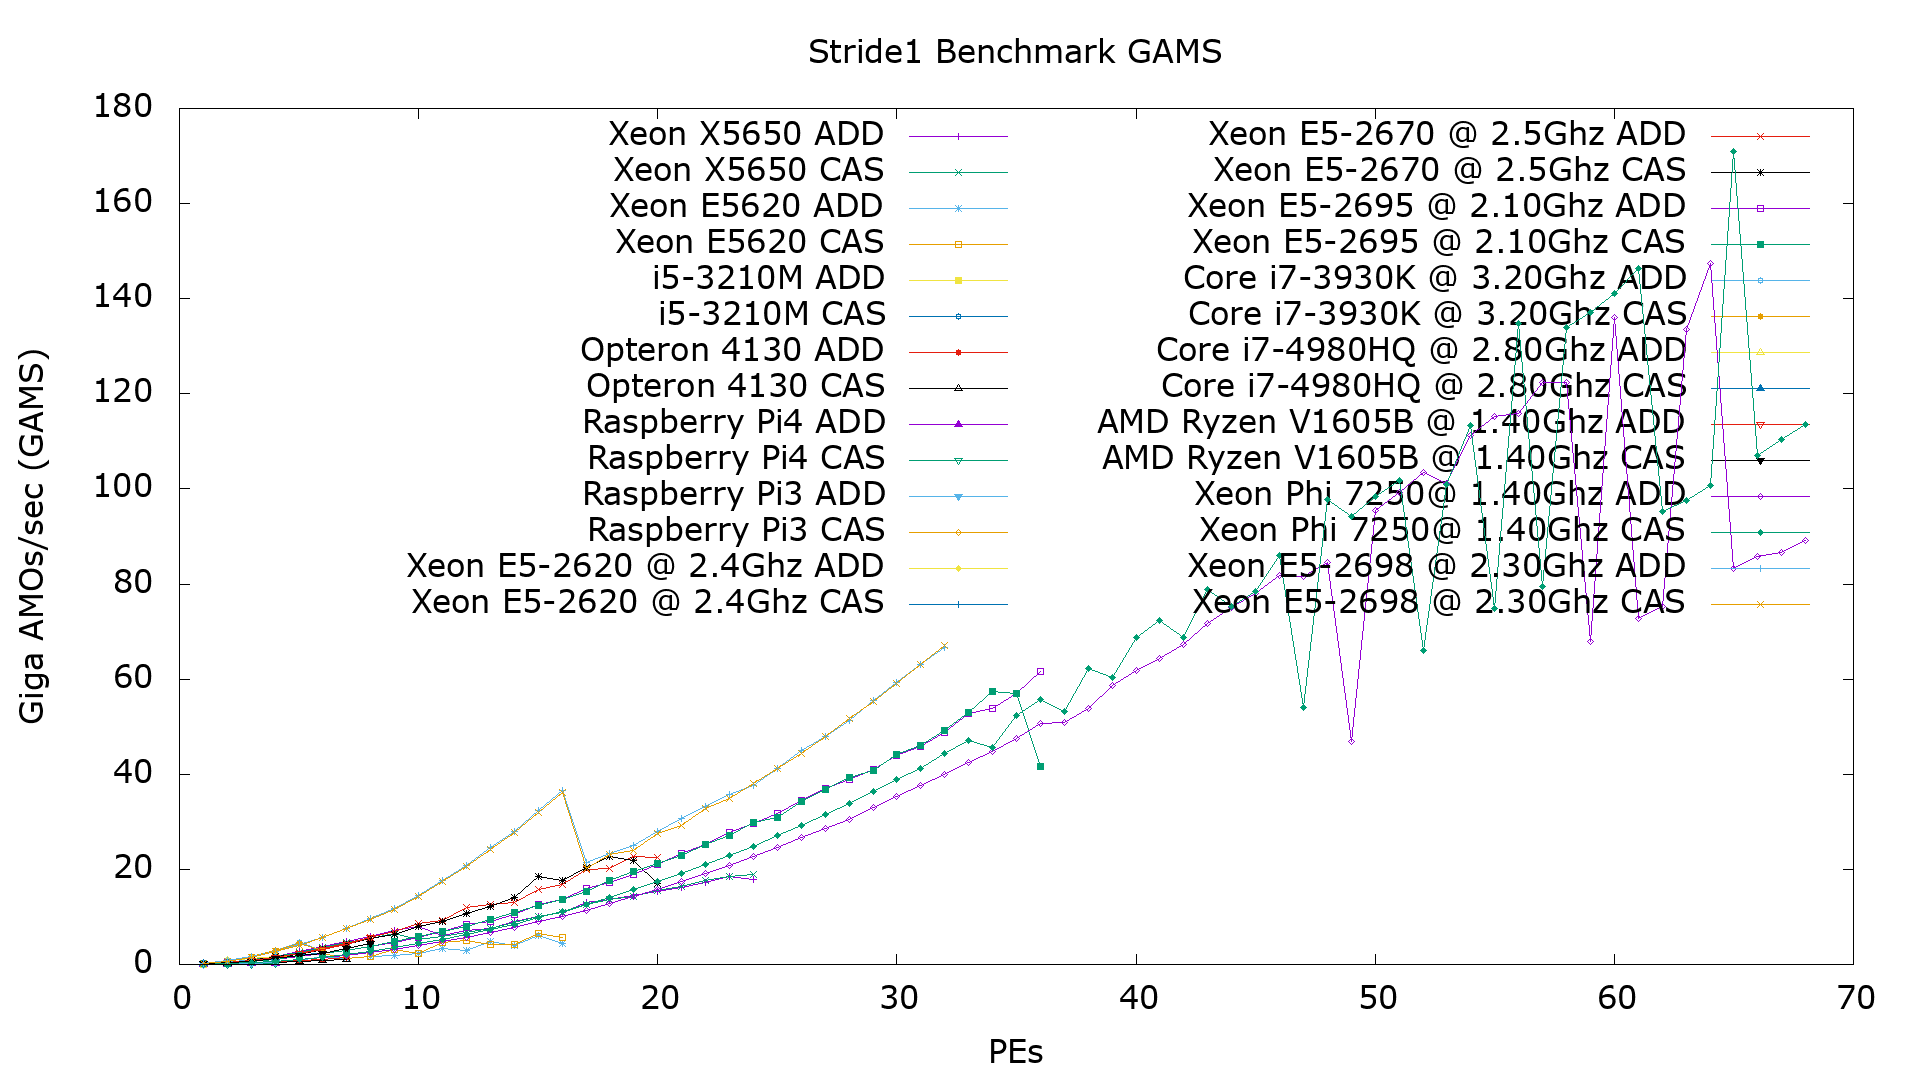
\includegraphics[width=3.5in]{figures/STRIDE1_GAMS.png}
\caption{Stride-1 Benchmark GAMS}
\label{fig:s1_gams}
\end{figure}

Our results for the Stride-1 kernel benchmark, shown in Figure~\ref{fig:s1_gams}, clearly contrast with those of the previous kernel.
Herein, we see a marked improvement in the \textit{GAMs} performance of the majority of our test platforms.
This divergence is particularly prominent for some of our more powerful platforms such as the Xeon E5 class systems and the Core i7-3930k.
However, the Core i7-4980HQ platform, which performed poorly in the Random Access benchmark, also makes unmistakable improvements.
Orthogonally, the Core i5-3210M system performs much more poorly in comparison.
Similar to the previous benchmark, a noticeable dip in performance occurs at 17 threads for the Xeon X5-2698 v3 system.
Unlike the Random Access benchmark, there is little discernible performance variation between CAS and Add kernel implementations within a platform.
For this benchmark, some unusual behavior is also demonstrated by the Xeon Phi 7250 platform, wherein the performance becomes erratic around 46 threads.
We detail our conclusions in regard to this system in Section~\ref{subsubsec:new_insights}.

\subsubsection{Stride-N}
\label{subsubsec:striden_res}

\begin{figure}[!t]
\centering
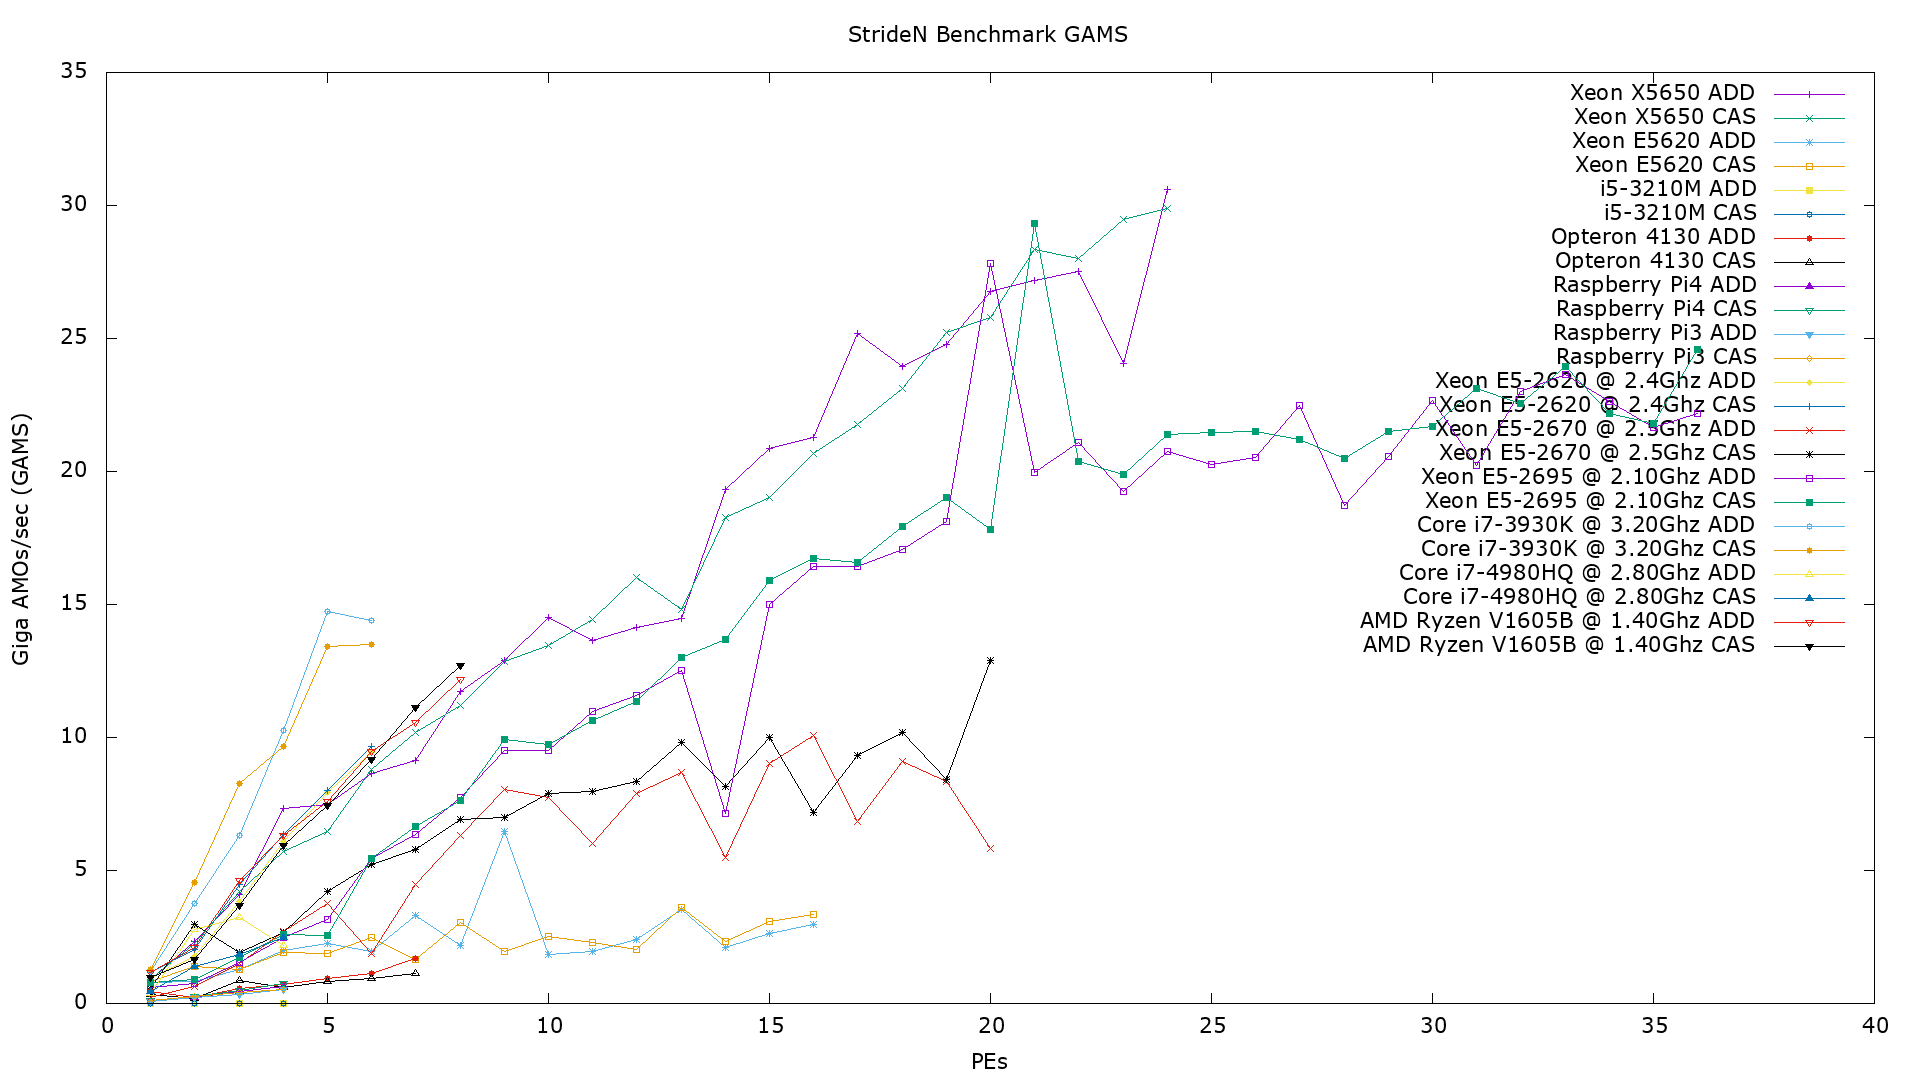
\includegraphics[width=3.5in]{figures/STRIDEN_GAMS.png}
\caption{Stride-N Benchmark GAMS}
\label{fig:sn_gams}
\end{figure}

The results of our Stride-N kernel benchmark, illustrated in Figure~\ref{fig:sn_gams}, align most closely with those demonstrated by the Stride-1 benchmark.
Here, the \textit{GAMs} performance exhibited by each platform is much higher than it was for the Random Access kernel.
Indeed, the \textit{GAMs} recorded for this kernel often exceed those shown for the Stride-1 kernel.
We attribute this behavior to the fact that each thread operates most often on distinct memory segments within this kernel.
This improves each thread's private cache utilization while minimizing cache line invalidations.
It also explains the absence of the cross-socket performance degradation demonstrated by the Xeon E5-2698 v3 system in other kernel benchmarks.
The platforms that performed well during the Stride-1 benchmark, such as the Core i7-3930k and Xeon E5-2698 v3 systems, also exhibit impressive performance for this kernel.
Our Ryzen V1605B platform also performs well in comparison.
Likewise, those that performed poorly in the Stride-1 benchmark, including the Opteron 4130 and Cortex systems, often replicate that behavior here.
In fact, the Core i5-3210M system manifests the poorest performance in this benchmark across all tested platforms.
Also similar to the Stride-1 benchmark, with the exception of the Xeon Phi 7250 system, very little performance variation is measured between the CAS and Add kernel implementations.
Orthogonal to the Stride-1 benchmark, there appears to be a hard upper bound in regard to the scalability of each platform for this kernel.
Given the behavior of this kernel and our demonstrated results, we ascribe this bound to be a function of each platform's cache size.
The presence of the on-package 16GiB MCDRAM, configured as a last-level cache, may also help explain why this generalization does not apply to the CAS kernel implementation on the Xeon Phi 7250 platform.

\subsubsection{Pointer Chase}
\label{subsubsec:ptrchase_res}

\begin{figure}[!t]
\centering
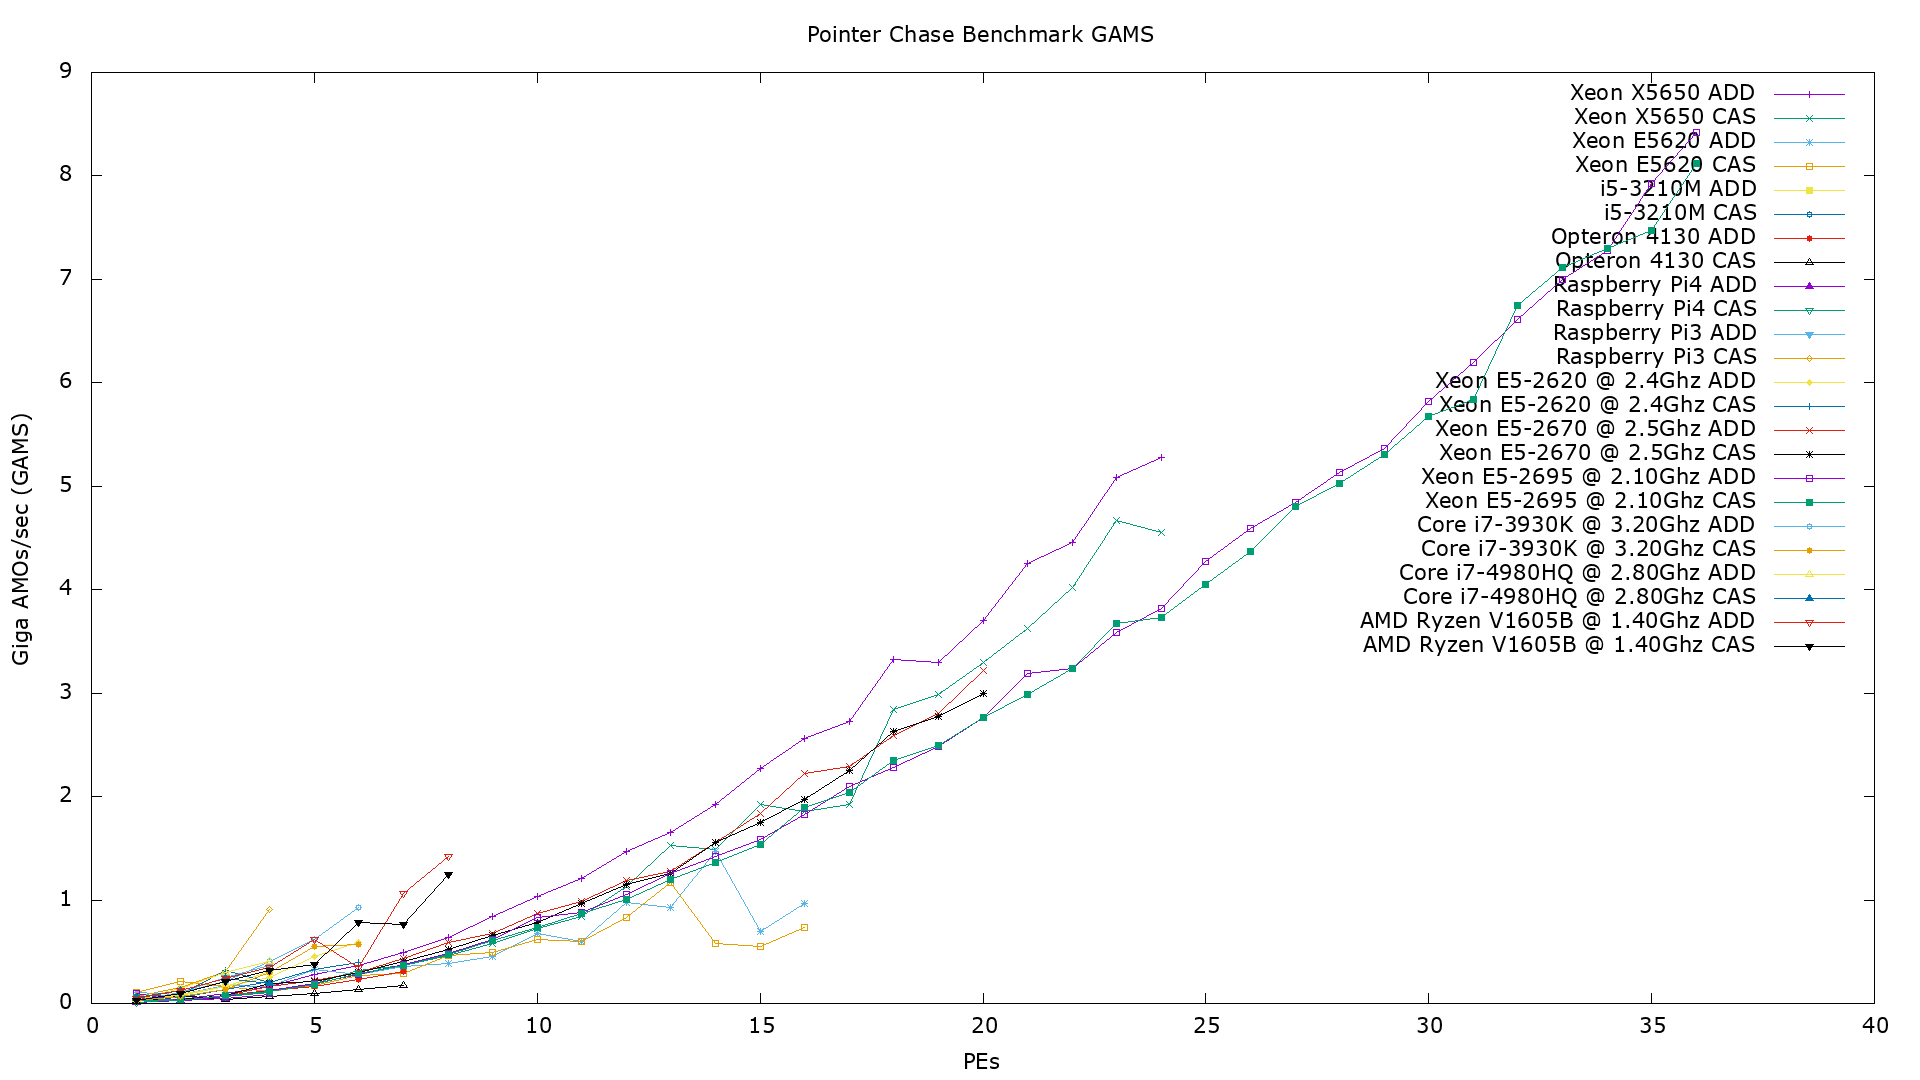
\includegraphics[width=3.5in]{figures/PTRCHASE_GAMS.png}
\caption{Pointer Chase Benchmark GAMS}
\label{fig:ptrchase_gams}
\end{figure}

We next investigate the results of our Pointer Chase kernel benchmark.
As shown in Figure~\ref{fig:ptrchase_gams}, the \textit{GAMs} performance for this kernel across platforms is lower than each of the previously detailed benchmarks.
Similar to the Random Access kernel, this kernel exhibits irregular, unpredictable memory access patterns.
However, in contrast to the Random Access kernel, the Pointer Chase kernel performs atomic operations to memory locations within the \texttt{IDX} array.
Since the size of this array is based on a static calculation, and is typically much smaller than the \texttt{VAL} array, this behavior results in an increased number of cache line invalidations and associated cache misses. 
Consequently, the ability of the cache to improve system performance is severely diminished.
As a result, the benefits to performance offered by large caches are effectively nullified in this benchmark and, in most cases, our more powerful systems perform little better than their counterparts for the same number of threads.
Notably, the Xeon Phi 7250 platform almost uniformly records the lowest \textit{GAMs} performance regardless of thread count.
Further, its erratic behavior as the number of threads increases, as noted for other kernels, is particularly prominent in this benchmark and begins at a much lower number of threads.
The results from this benchmark are also the first to showcase a distinct performance benefit for atomic Add based kernel implementations as compared to CAS implementations.

\subsubsection{Central}
\label{subsubsec:central_res}

\begin{figure}[!t]
\centering
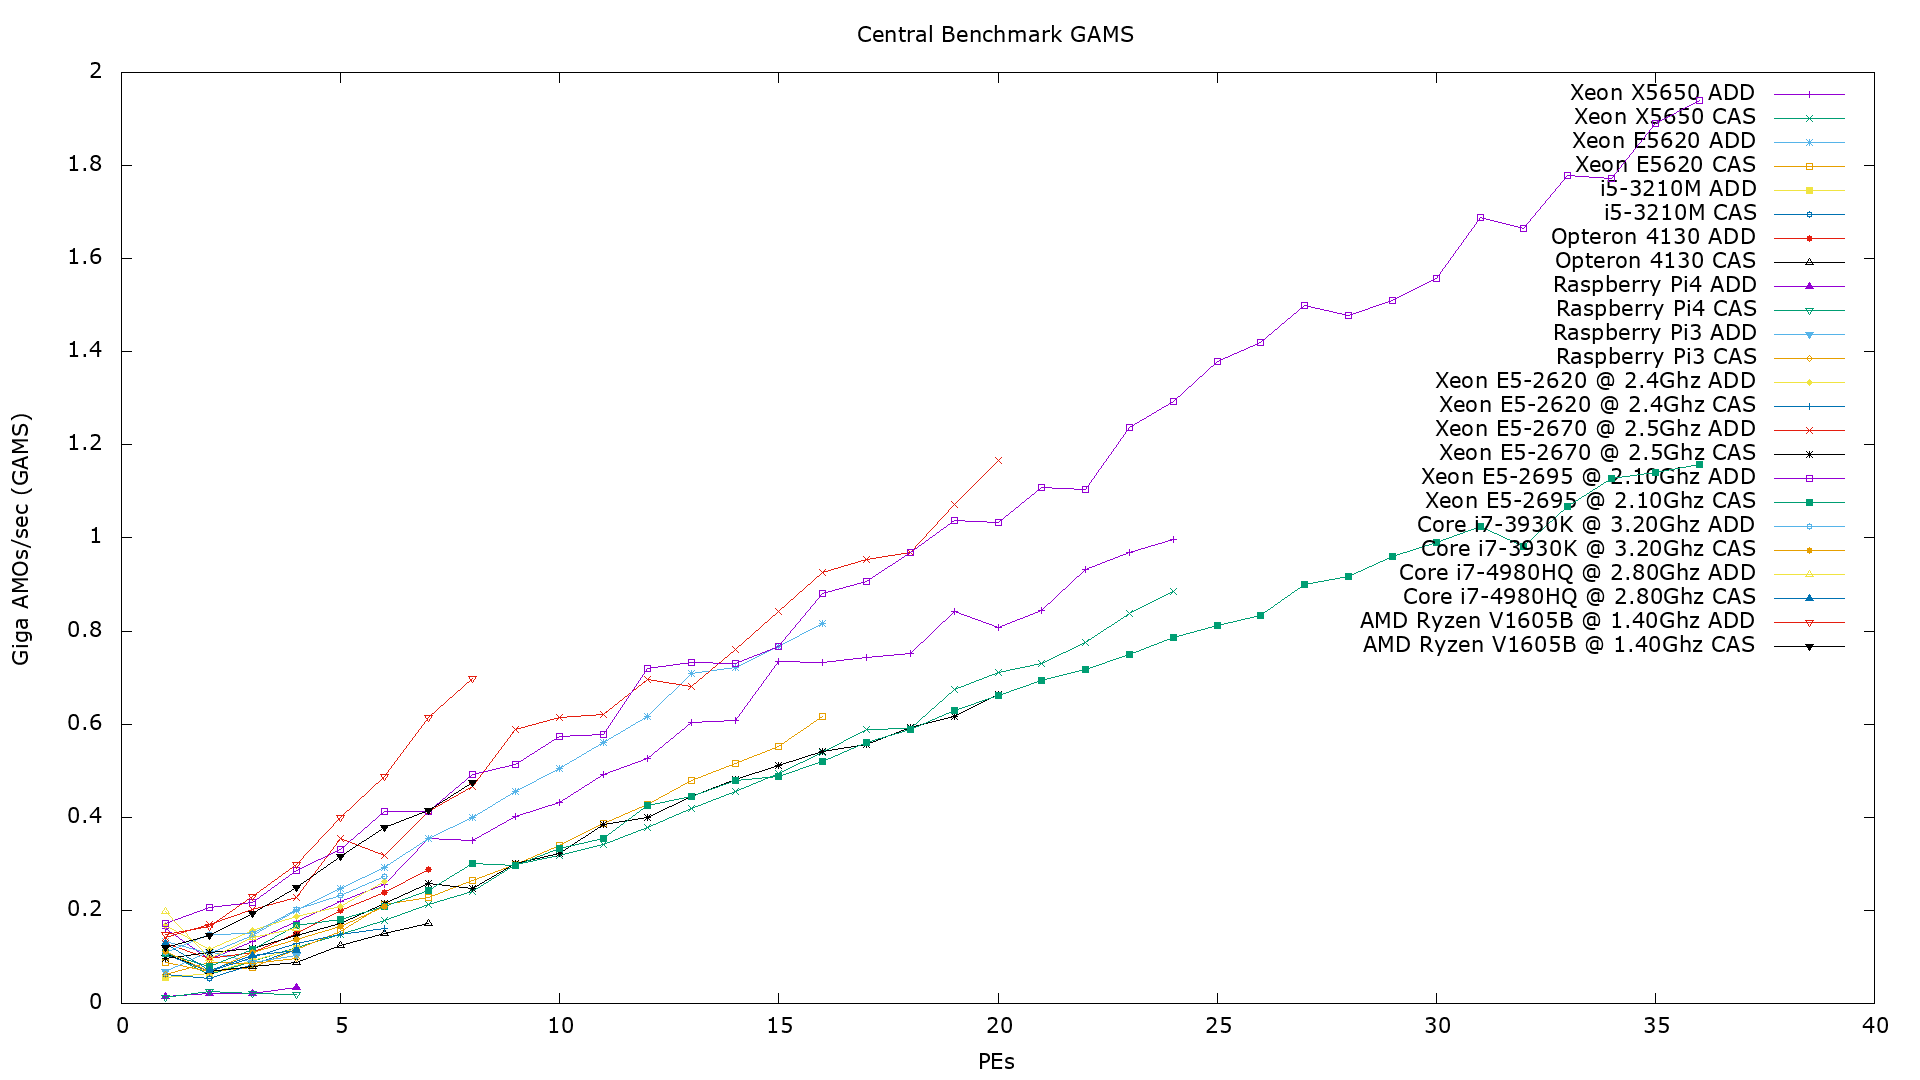
\includegraphics[width=3.5in]{figures/CENTRAL_GAMS.png}
\caption{Central Benchmark GAMS}
\label{fig:central_gams}
\end{figure}

Although the Random Access and Pointer Chase kernels perform more poorly than the Stride-1 and Stride-N kernels, the \textit{GAMs} measured in our Central kernel benchmark, as shown in Figure~\ref{fig:central_gams}, are by far the lowest of any in the CircusTent suite.
As each thread performs an atomic operation to a common memory location during each iteration of the kernel loop, the measured \textit{GAMs} performance for this kernel is directly dependent on the characteristics of a target architecture's memory subsystem.
Since the number of requests any memory hierarchy can service within a given time frame is limited, the \textit{GAMs} performance of this kernel for a given platform will eventually plateau as the number of PEs increases.
Although several of our systems, such as the Xeon E5 class systems, may not have reached their zenith, our results demonstrate that many of our other platforms quickly reach such a plateau.
Indeed, none of our test platforms ever exceed 2 \textit{GAMs} in this benchmark.
As contention for memory access represents a limiting factor in this benchmark, other components that contribute to a system's performance are less visible in these results.
This explains the absence of any cross-socket performance decline for the Xeon E5-2698 v3, or any other, platform.
In addition to our Xeon E5 platforms, which continue to perform well across disparate kernels, our Ryzen V1605B system also registers exceptional performance in this benchmark.
In fact, the Ryzen system has the highest \textit{GAMs} performance of any platform for 4 or fewer threads.
In contrast, our Cortex-A72, Cortex-A53, Xeon Phi 7250, and Core i5-3210M systems again represent the lowest performers for this benchmark.
However, the Opteron 4130 platform performs slightly better than in previous trials.
Similar to the Pointer Chase kernel, the Central kernel seems to elicit higher performance from atomic Add implementations.

\subsubsection{Scatter}
\label{subsubsec:scatter_res}

\begin{figure}[!t]
\centering
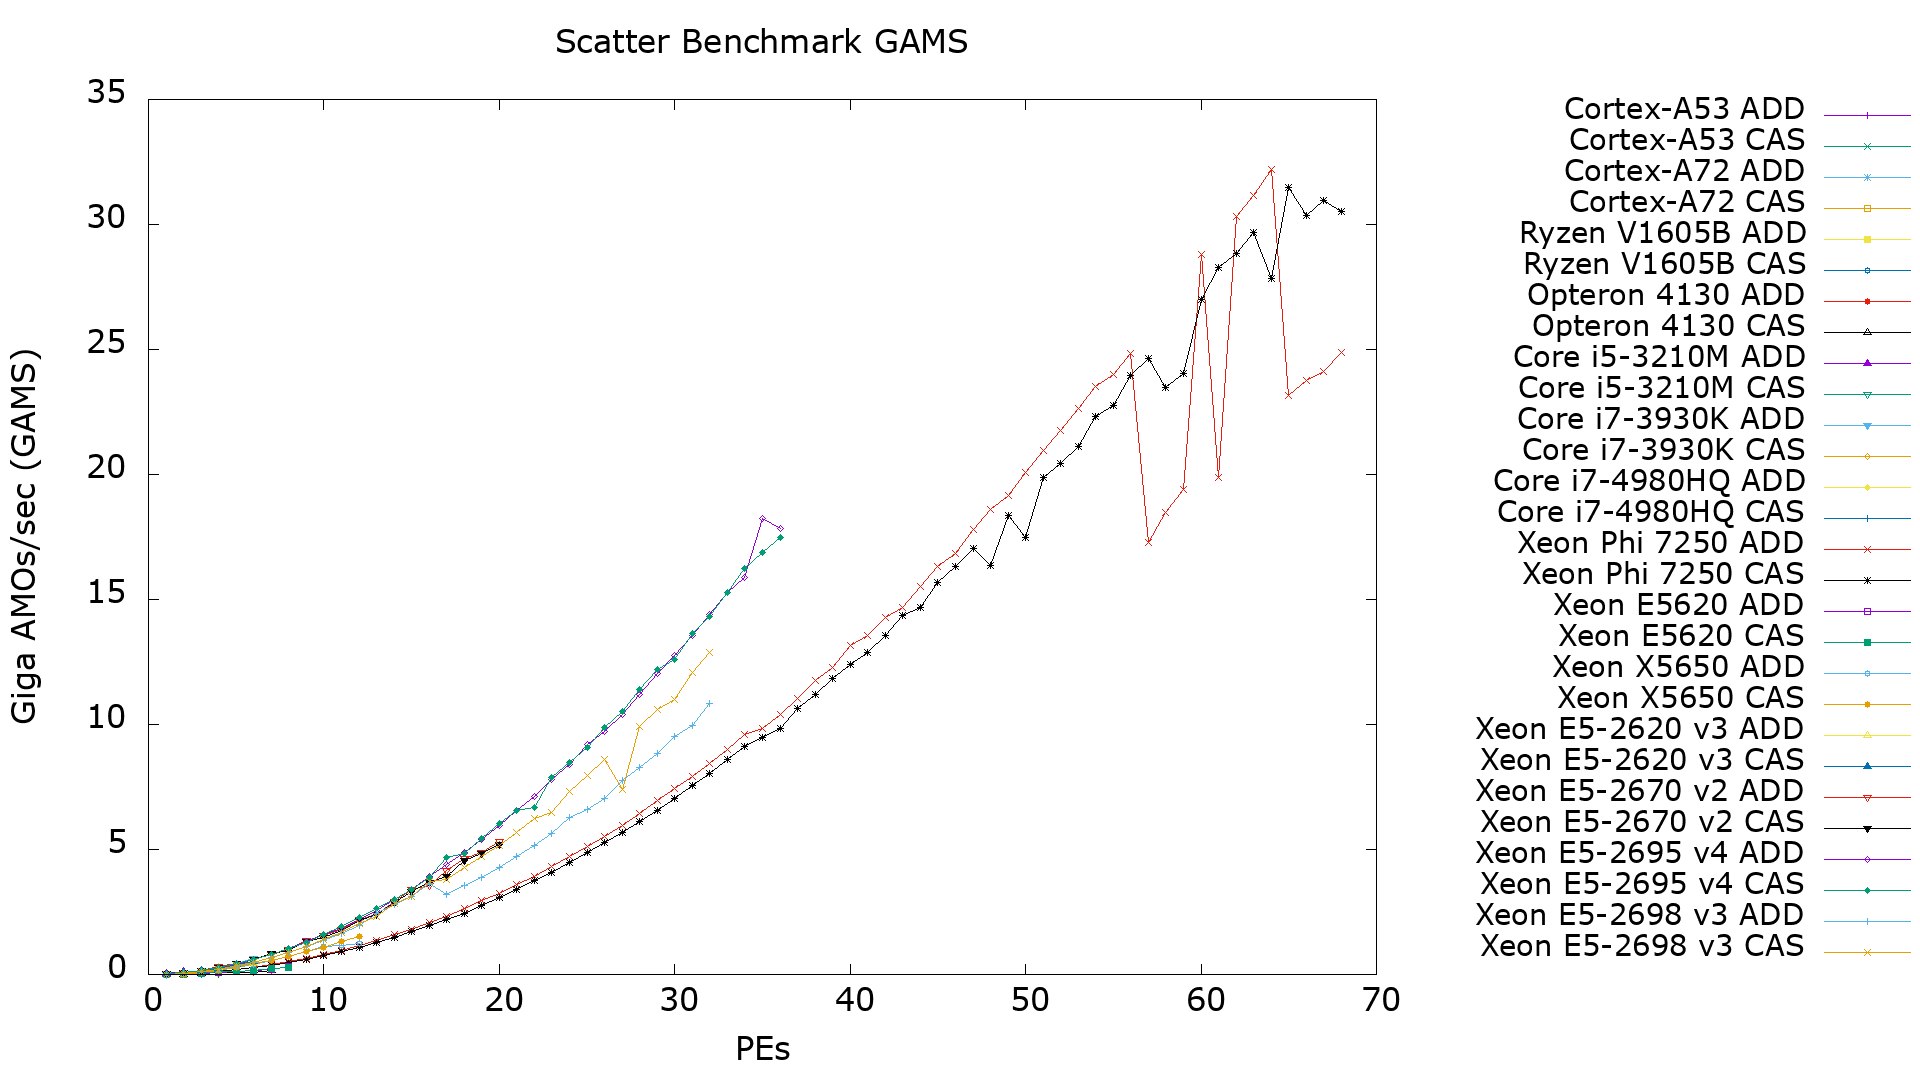
\includegraphics[width=3.5in]{figures/SCATTER_GAMS.png}
\caption{Scatter Benchmark GAMS}
\label{fig:scatter_gams}
\end{figure}

The results for our Scatter kernel benchmark are shown in Figure~\ref{fig:scatter_gams}.
The most immediately observable characteristic of this graph is the steadily increasing performance of each platform as the number of threads increases.
The only major exception to this behavior is manifested by the Xeon Phi 7250 system beyond approximately 56 threads.
Another observation can be made in regard to the relative performance of our test platforms in this benchmark.
In general, each system exhibits improved performance as compared to the Random Access and Pointer Chase benchmarks, but poorer performance compared to the Stride-1 and Stride-N benchmarks.
Given what we know about the memory access patterns of these previous kernels, these results imply that the indexed access patterns present in the Scatter kernel are able to leverage the cache hierarchy to improve performance to some degree.
The higher performance exhibited by our Xeon and Core i7-3930k systems lend some credence to this conclusion.
However, the fact that our Core i5-3210M platform records the highest \textit{GAMs} across all tested platforms suggests other factors may also play a role.
Moreover, the poor performance of the Core i7-4980HQ system, which features an L4 cache in addition to a conventional L3, further increases this likelihood.
Another notable characteristic of this kernel is that our Xeon e5-2698 v3 platform again experiences a drop in performance associated with cross-socket thread placement.
However, this behavior only occurs for the atomic Add kernel implementation.
Whereas other kernels demonstrated often demonstrated improved performance for a particular atomic primitive, the Scatter kernel seems to perform equally well for either CAS or Add kernel implementations.

\subsubsection{Gather}
\label{subsubsec:gather_res}

\begin{figure}[!t]
\centering
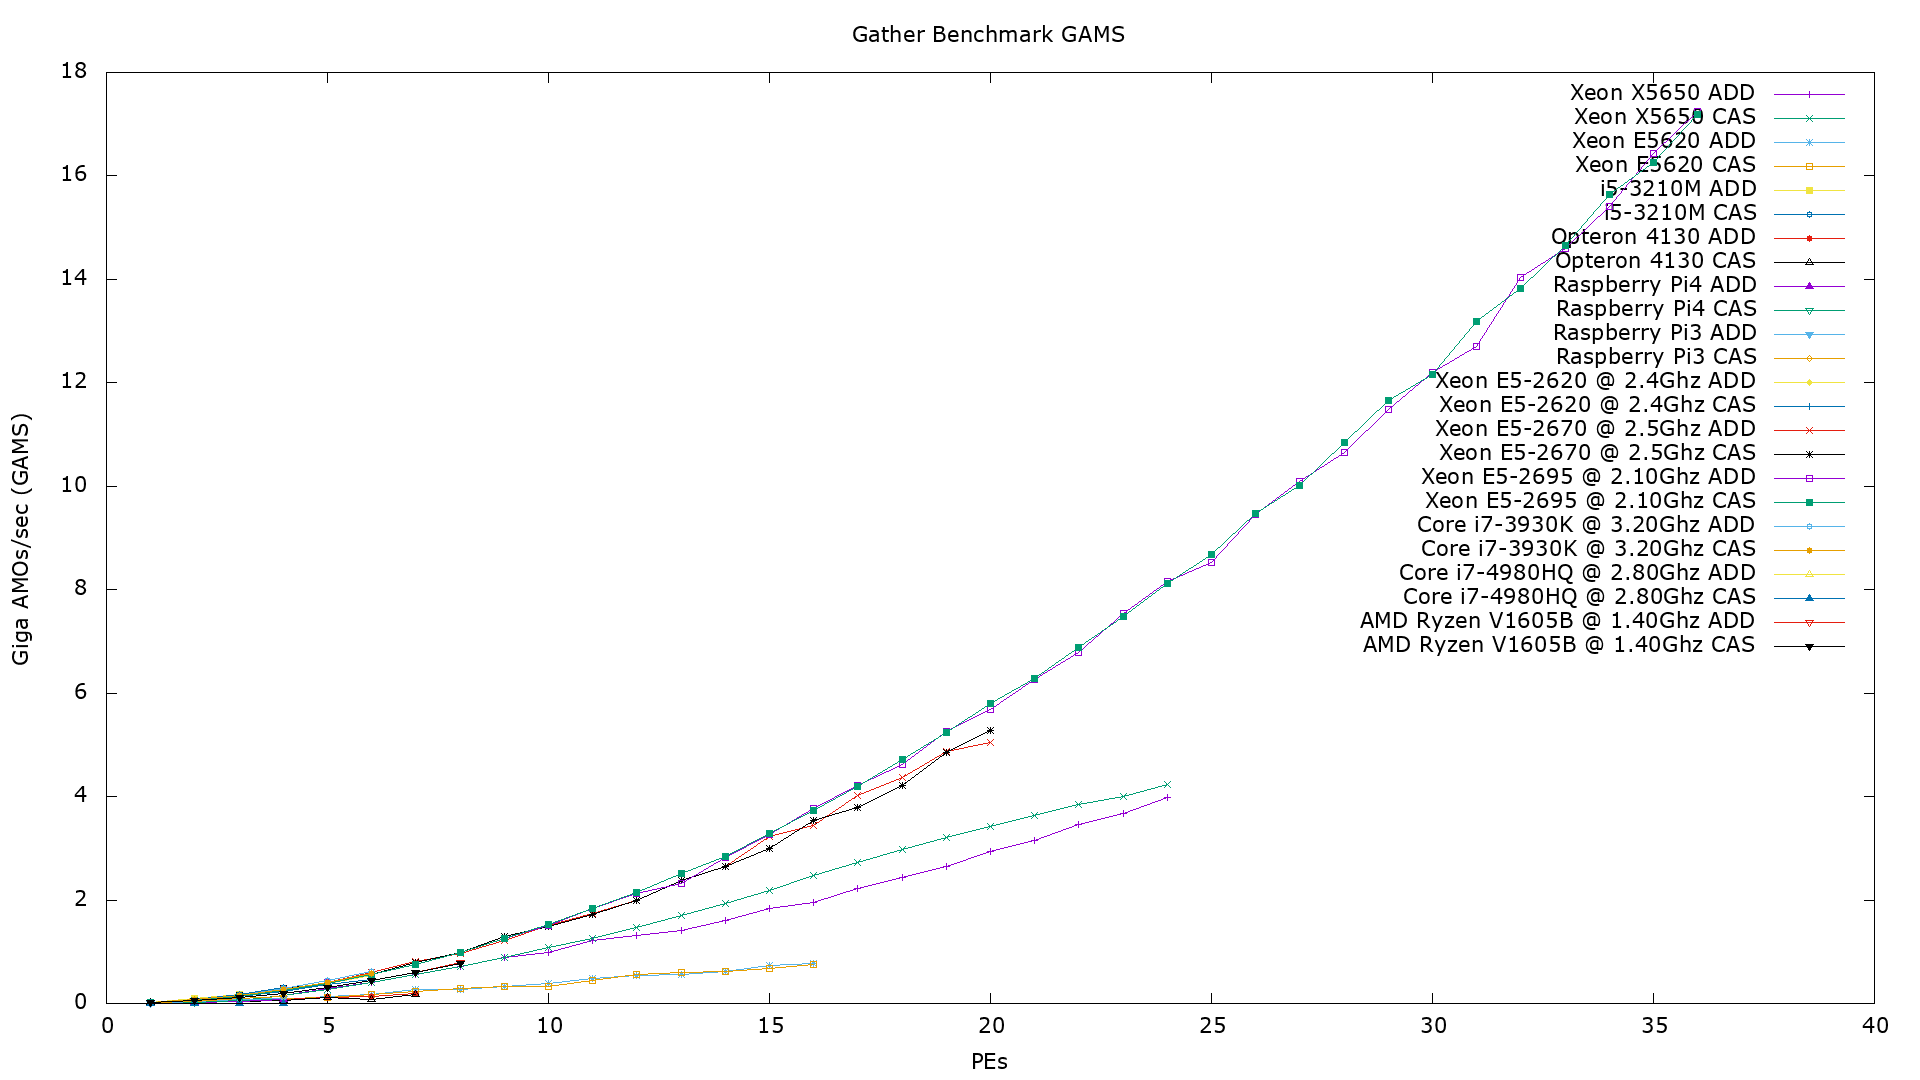
\includegraphics[width=3.5in]{figures/GATHER_GAMS.png}
\caption{Gather Benchmark GAMS}
\label{fig:gather_gams}
\end{figure}

Given the relationship between the Scatter and Gather kernels, it is unsurprising that our Gather benchmark results share many similarities with those detailed in Section~\ref{subsubsec:scatter_res}.
In fact, as shown in Figure~\ref{fig:gather_gams}, the \textit{GAMs} performance across platforms for this kernel closely emulate those exhibited by the Scatter kernel.
Both benchmarks demonstrate the same predictable improvement to the measured \textit{GAMs} performance as the number of threads increases.
Further, the \textit{GAMs} performance of given a platform in the Gather benchmark is approximately equivalent to its performance in the Scatter benchmark.
For our Xeon E5-2698 v3 platform, the now familiar cross-socket performance decline is also replicated only for the atomic Add implementation of the Gather kernel.
With the exception of this system, the performance of the Gather kernel is likewise comparable for atomic Add and CAS implementations across systems and thread counts. 
Perhaps the most readily visible difference between the two sets of results is the fact that the erratic performance characteristics associated with our Xeon Phi 7250 system begin at a lower thread count in the Gather benchmark.

\subsubsection{Scatter/Gather}
\label{subsubsec:sg_res}

\begin{figure}[!t]
\centering
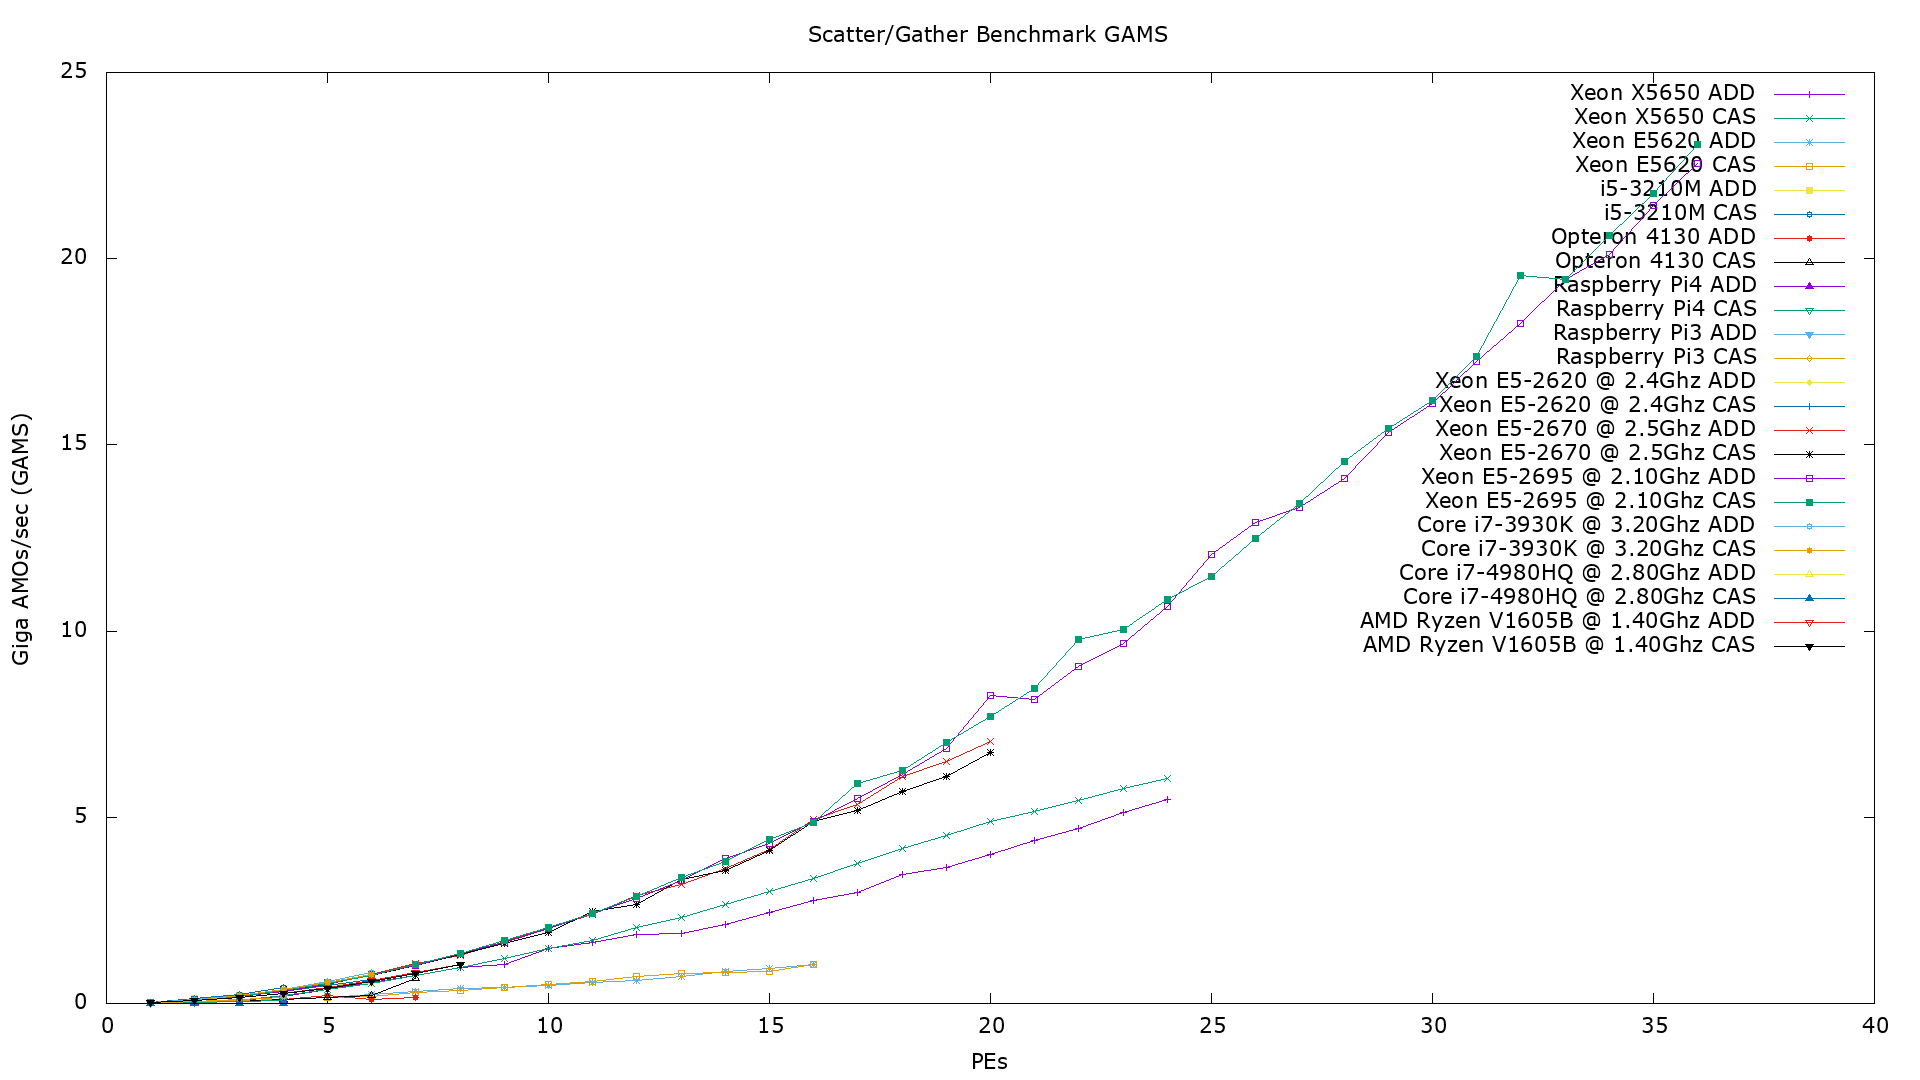
\includegraphics[width=3.5in]{figures/SG_GAMS.png}
\caption{Scatter/Gather Benchmark GAMS}
\label{fig:sg_gams}
\end{figure}

The results of our final benchmark, performed using the Scatter/Gather kernel, are shown in Figure~\ref{fig:sg_gams}.
As might be expected, the results for this kernel are highly congruous with those demonstrated by the individual Scatter and Gather benchmarks.
The same cross-socket behavior exhibited by our Xeon E5-2698 v3 platform in these benchmarks is repeated for the Scatter/Gather kernel.
Similarly, the Scatter/Gather kernel does not display an affinity for either atomic Add or CAS kernel implementations.
Notably, however, the \textit{GAMs} performance across platforms for this benchmark is slightly improved as compared to the Scatter and Gather benchmarks.
This behavior is particularly pronounced at higher thread counts and for our more powerful platforms.
As such, we conclude that the combination of the Scatter and Gather memory access patterns within a single kernel leads to an improved cache hit rate as the level of concurrency rises.
Our Core i5-3210M system again manifests surprisingly impressive performance in this benchmark.
However, the otherwise dominant performance of our Xeon and Core i7-3930k systems further support our conjecture.
As with the Scatter and Gather benchmarks, our Core i7-4980HQ system presents exceptionally poor performance for this kernel.
The Cortex-A72, Opteron 4130, and Xeon E5620 systems round out the lowest performing platforms for this benchmark.

\subsection{Analysis}
\label{subsec:analysis}

\subsubsection{Expected Correlations}
\label{subsubsec:expected_correlations}

In many ways, the results gathered during our CircusTent evaluation conform to expectations.
The variance of \textit{GAMs} performance across different kernels, regardless of platform, is one such example.
Here, the measured performance is highest in kernels that utilize uniform memory access patterns, such as the Stride-N and Stride-1 kernels.
These uniform access patterns leverage the principle of spatial locality to service a higher percentage of memory requests from the cache.
As such, they improve performance for atomic operations in much the same manner that they do so for traditional loads/stores.
In contrast, kernels that utilize unpredictable memory access patterns are often forced satisfy requests from main memory.
Accordingly, the recorded \textit{GAMs} performance of the Random Access and Pointer Chase kernels is much lower.
The performance of the Scatter, Gather, and Scatter/Gather CircusTent kernels, which utilize semi-random, indexed access patterns, falls between these two classifications.
Predictably, the Central kernel, wherein concurrent atomic operations to a single memory location are repeatedly performed, exhibits the lowest performance and quickly reaches an upper bound as the degree of contention rises.

A similar generalization can be made in regard to the correlation between cache size and platform performance.
Notably, the systems that sustain the highest \textit{GAMs} performance across the distinct CircusTent kernels, such as the Xeon E5-2670 v2, Xeon E5-2695 v4, and Xeon E5-2698 v3, correspond to the those that feature the largest last-level caches.
In contrast, the systems that often exhibit the poorest performance, including the Cortex-A53, Cortex-A72, and Opteron 4130, typically feature much smaller caches.
This disparity directly illustrates the benefits a large cache size offers for atomic operation performance.
These observations, consistent with conventional architectural wisdom, increase our confidence in the correctness and viability of the CircusTent benchmark suite.

\subsubsection{New Insights}
\label{subsubsec:new_insights}

Our CircusTent evaluation also provides some new insights into the performance of atomic operations that are not readily apparent.
The unexpectedly higher performance of our CAS kernel implementations over their atomic Add analogs in some scenarios is one such example.
Conventional wisdom dictates that the data overheads associated with the CAS instruction render it less efficient than other atomic instructions such as Add.
However, our test platforms uniformly measured higher \textit{GAMs} performance for the CAS implementation of the CircusTent Random Access kernel.
We attribute this behavior to several contributing factors.
First, our OpenMP Random Access kernel implemented using the CAS atomic primitive is written such that the value of \textit{VAL[IDX[i]]} is compared against itself to determine the proper store value.
In the event the values are equivalent, which is always the case for this implementation, the CAS instruction again stores this same value to the specified location.
Herein, it is likely that the microarchitecture recognizes that the value to be written and the value already stored are, in fact, the same and optimizes performance by skipping the store component of the CAS operation.
In this case, the time taken to execute each CAS instruction is reduced in a manner that the Add instructions are not.
Further, writing the same value into each memory location during successive iterations of the kernel loop prevents cache-line invalidations.
In scenarios wherein cache blocks are present in multiple private caches, this directly improves overall performance by increasing the cache-hit rate at higher levels of the cache hierarchy.  
Taken together, these behaviors explain the apparent performance discrepancy between the CAS and ADD implementations.
Moreover, these observations suggest that future compilers may be able to further optimize performance by replacing atomic Add instructions with CAS analogs when values are expected to be modified infrequently.

We also observe that the performance characteristics of two of our test platforms deviate from our expectations.
Since our Core i7-4980HQ system features a 128 MiB shared L4 cache in addition to its L3, we anticipated that this platform would be one of the higher performers across kernels.
For four of our benchmarks, however, this system generated only mediocre \textit{GAMs} performance that seems more inline with its 6MiB L3 cache.
Further, in our Random Access, Scatter, Gather, and Scatter/Gather benchmarks, it was by far the poorest performing platform.
Given the random memory access patterns inherent in these kernels, it seems likely that many cache lines would be evicted from the L3 cache into the L4 during benchmark execution.
Although we assume the eDRAM-based L4 cache has a higher latency than its SRAM counterparts, it would still be expected to service requests faster than main memory.
As such, we are currently exploring the microarchitecture of this system's memory hierarchy to better understand these results.

The performance of our Xeon Phi 7250 platform was also somewhat surprising.
Although the cores present on this processor do not share a true last-level cache, we anticipated the 16GB of MCDRAM operating in the cache configuration to appreciably improve the performance of this platform.
However, when compared to trials performed on other systems with equivalent thread counts, the Xeon Phi 7250 system performed poorly across the disparate set of CircusTent kernels.
Moreover, its performance in many benchmarks was abnormally erratic.
Notably, this behavior became increasingly aggravated as the thread count rose and was particularly prominent in our Stride-1 and Pointer Chase benchmark results.
We believe this system's erratic behavior and sub-par performance can be attributed to several factors associated with its complex memory subsystem.
First, the absence of a true-last level cache on this platform directly entails some degree of performance degradation.
As the L1 and L2 caches on this system cannot cache all the necessary information, requests must often be serviced from the MCDRAM.
Although one might expect this MCDRAM to improve performance in comparison to main memory, the opposite effect occurs.
Here, the increased latency of the MCDRAM combined with the irregular memory access patterns exhibited by the CircusTent kernels diminish the platform's performance~\cite{peng2017exploring}.
As such, any requests that would be serviced by the L3 cache, or even main memory, on other systems often incur a significant penalty for the Xeon Phi 7250 platform.
Second, and perhaps even more importantly, the 34 L2 caches resident on each tile in this processor are kept fully coherent.
As any invalidation for shared cache lines must be propagated across this complex system, these operations are exceedingly costly.
These expensive operations, combined with the fact that any core possessing an invalidated cache line must then service a subsequent request from the MCDRAM, make shared cache lines across cores not resident within the same tile an expensive proposition for this system.
As execution with an increasing thread count, as well as the Stride-1 and Pointer Chase kernels themselves, represent scenarios wherein cache line sharing is progressively likely, we feel this reinforces our conclusion regarding the performance of this platform.
Further, this behavior can also explain the variation between the performance of the CAS and Add Stride-N kernel implementations.
As our Stride-N CAS implementation operates in the same manner as the Random Access implementation previously detailed, cache line invalidations are similarly not generated in this benchmark.
Thus, the absence of these invalidations allows the CAS implementation to far surpass that of the atomic Add implementation on our Xeon Phi 7250 platform.

Beyond the considerable impact cache size and organization has on atomic operation performance, the operating system and compiler may play a bigger role than originally anticipated.
For example, we observe that our Ryzen V1605B system performs significantly better than expected in several of our kernel benchmarks despite its modest cache size.
As we have not yet been able to isolate any microarchitectural factors that would explain this anomaly, it may be a result of the newer operating system and compiler used on this platform.
While our Core i5-3210M also exceeds expectations in several benchmarks, we suspect this performance may be a function of the smaller \texttt{VAL} array utilized on this system.
As our Xeon E5620 system performed significantly more poorly than similar systems with identical cache organizations, the operating system and compiler may also be at fault here.
Finally, we note that while our Xeon E5-2698 v3 system demonstrated cross-socket performance degradations in several of our benchmarks, none of our other dual-socket platforms manifested the same behavior.
Despite our efforts to avoid simultaneous multithreading, it is possible the operating systems of these platforms attempted to optimize performance by scheduling threads to the same physical core rather than cross socket boundaries.